\documentclass{article}
\usepackage{pgfplots}
\usepackage{filecontents}
\usepackage{verbatim}
\pgfplotsset{compat=1.8}
\usepackage{pgfplotstable}

\begin{document}
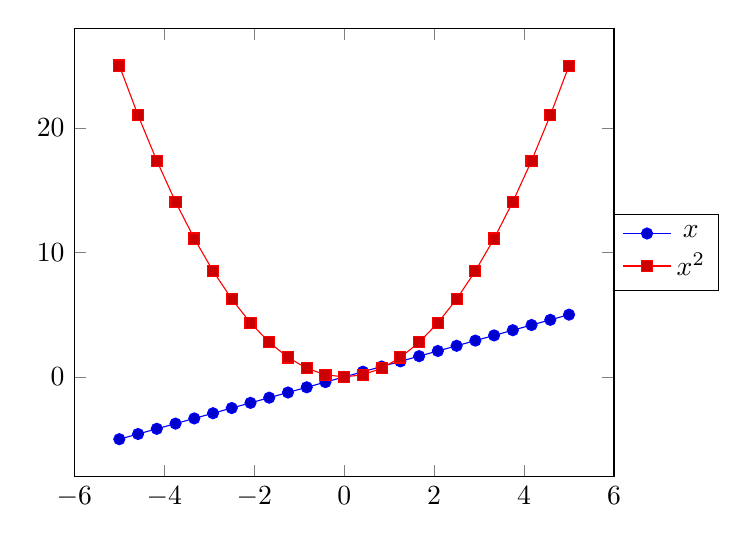
\begin{tikzpicture}
  \begin{axis}[
      legend entries={$x$,$x^2$},
      legend style={
        at={(1,0.5)},        % 1.03(>1) moves out of the graph along x, 0.5 means half-way along y
        anchor=west         %where the image will 'hang/support'. North/South/East/West means anchor will attach at ``at coordinate from top/bottom/right/left that direction. 
      }
    ]
    \addplot {x};
    \addplot {x^2};
  \end{axis}
\end{tikzpicture}

\setlength{\fboxsep}{0pt}
\fbox{
  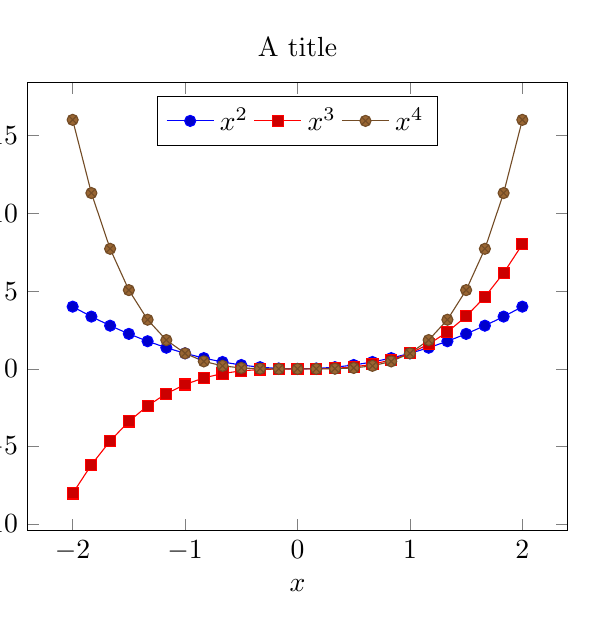
\begin{tikzpicture}
    \begin{pgfinterruptboundingbox}
      \begin{axis}[
          title=A title,
          xlabel={$x$},
          ylabel={$y$},
          legend style={at={(0.5,0.97)},
            anchor=north,legend columns=-1},
          domain=-2:2           % domain on the x axis
        ]
        \addplot {x^2};
        \addplot {x^3};
        \addplot {x^4};
        \legend{$x^2$,$x^3$,$x^4$}
      \end{axis}
    \end{pgfinterruptboundingbox}

    \useasboundingbox
    (current axis.below south west)
    rectangle (current axis.above north east);
  \end{tikzpicture}
}

\begin{tikzpicture}
  \begin{axis}[%
      scale only axis,
      width=0.45\textwidth,
      height=0.2\textheight,
      xmin=0, xmax=300,
      ymin=-2e+06, ymax=1e+07,
      legend entries={Analytic solution,GPS data,Kalman filtered},
      legend style={nodes=right},
      legend pos= south east]

    \addplot [color=blue, solid]
    coordinates{ (0,7e+06) (0.1,7.0007e+06) (0.2,7.0014e+06) };

    \addplot [color=green, solid]
    coordinates{ (0,6.99999e+06) (0.1,7.00071e+06) (0.2,7.00143e+06) };

    \addplot [color=red, solid]
    coordinates{ (0,0) (0.1,7.00071e+06) (0.2,7.00174e+06) };

  \end{axis}
\end{tikzpicture}


\begin{comment}
  :Title: Convergence Plot
  :Tags: PGFPlotstable;Mathematics;Manual
  :Author: Christian Feuersänger
  :Slug: convergence-plot

  We assume that we did some scientfic experiment.
  The scientific experiment yielded three
  input data tables: one table for each involved parameter
  d = 2, d = 3, d = 4. The data tables contain ``degrees
  of freedom'' and some accuracy measurement ``l2_err''. In addition,
  they might contain some meta-data
  (in our case a column ``level'').

  What we want is to produce three plots, each dof versus l2_err,
  in a loglog plot. We expect that
  the result is a line in a loglog plot, and we are interested in
  its slope log e(N) = -a log(N) because that
  characterizes our experiment.

  The code is from the PGFPlots 1.10 manual:
  ``3.3 Solving a Real Use Case: Scientific Data Analysis''.
\end{comment}
\begin{tikzpicture}
  \begin{loglogaxis}[
      title=Convergence Plot,
      xlabel={Degrees of freedom},
      ylabel={$L_2$ Error},
      grid=major,
      legend entries={$d=2$,$d=3$,$d=4$},
    ]
    \addplot table {../data/data_d2.dat};
    \addplot table {../data/data_d3.dat};
    \addplot table {../data/data_d4.dat};
    \addplot table[
      x=dof,
      y={create col/linear regression={y=l2_err,
            variance list={1000,800,600,500,400,200,100}}}
    ]
             {../data/data_d4.dat}
             % save two points on the regression line
             % for drawing the slope triangle
             coordinate [pos=0.25] (A)
             coordinate [pos=0.4]  (B)
             ;
             % save the slope parameter:
             \xdef\slope{\pgfplotstableregressiona}

             % draw the opposite and adjacent sides
             % of the triangle
             \draw (A) -| (B)
             node [pos=0.75,anchor=west]
             {\pgfmathprintnumber{\slope}};
  \end{loglogaxis}
  \begin{loglogaxis}[
      footnotesize,
      clip=false,
      xshift=7cm,
    ]
    \addplot table {../data/data_d2.dat}
    node [pos=1,pin=0:Special.] {}
    ;
  \end{loglogaxis}
\end{tikzpicture}

\end{document}
